\chapter{Router con QoS - Colas RED}
\label{chap:colasRED}

\section{Longitud de cola del router}

\subsection{Explica por qué se llenan tanto la cola AF1x como la AF2x pese a usar el algoritmo RED.} \label{chap:ejercicio411}
Como se puede ver en la gráfica \ref{fig:colasRED_tam} y en el archivo .ini de la práctica, la cola \textbf{AFX1} tiene un umbral máximo de 100 paquetes y la cola
\textbf{AFX2} tiene un umbral máximo de 50 paquetes. Además la probabilidad de descarte de paquetes es de 0,5 y 1 respectivamente en cada una.

Ambas colas tiene también un factor de suavizado que se usa para calcular el promedio de la longitud de la cola y ajustar dinámicamente la probabilidad
de descarte de paquetes. Cuanto menor sea este factor, el calculo de la longitud promedio de la cola se hará de forma mas lenta. 
Ese factor es de 0,03 en la cola \textbf{AFX1} y de 0,01 en la cola \textbf{AFX2}.

Como en este escenario hay una alta cantidad de paquetes entrantes, este factor de suavizado es muy bajo para este tráfico por lo que las colas tardan en detectar
la congestión y se llenan. Además en la cola \textbf{AFX1}, como la probabilidad de descarte es del 100\%, cuando la cola se llena se ve una
bajada muy grande en el tamaño, ya que en ese momento cualquier paquete que entre se descarta hasta que la cola quede estabilizada. 


\begin{figure}[!ht]
    \centering
    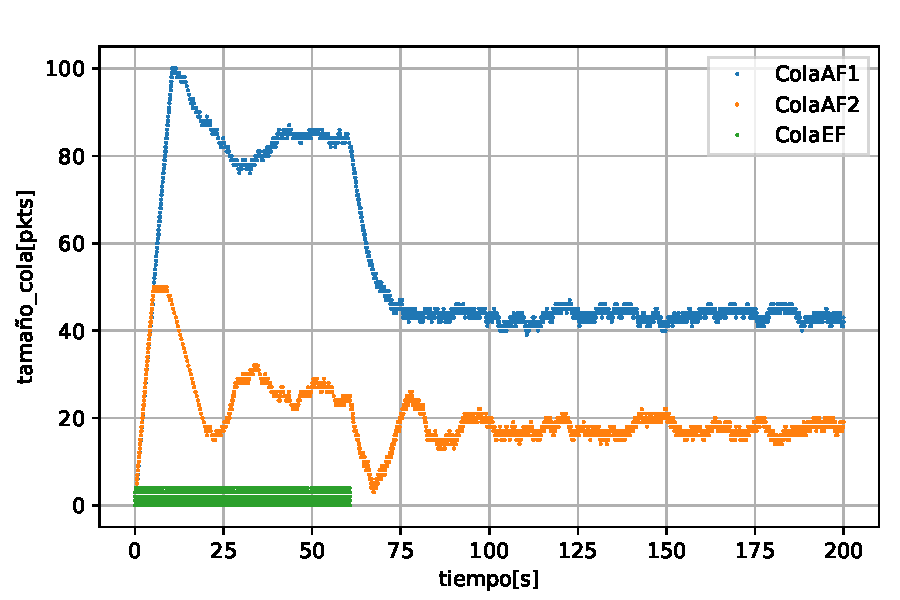
\includegraphics{graficas/RED/tamao_cola_red.pdf}
    \caption{Longitud cola del router con QoS usando colas RED}
    \label{fig:colasRED_tam}
\end{figure}


\subsection{Explica a qué es debida la bajada del tamaño de la cola AF2x:}
\begin{enumerate}
    \item Mientras dura la transmisión VoIP.
    
    Como se explicó en el apartado \ref{chap:ejercicio411}, al llenarse la cola la probabilidad de descarte es la máxima, por lo que se descartan
    todos los paquetes que llegan a la cola, bajando asi la congestión del tráfico.      

    \item Cuando ya no hay transmisión VoIP.
    
    A partir de los 60s se deja de transmitir paquetes VoIP entonces queda libre todo el ancho de banda para los paquetes UDP, 
    lo que hace que las colas estean ya menos congestionadas. Aún asi se ven subidas y bajadas en el tamaño de la cola (gráfica \ref{fig:colasRED_tam}) 
    ya que RED sigue descartando paquetes según el factor de suavizado, por lo que se aplica el límite según la longitud promedia de la cola (calculado en 
    el apartado \ref{text:calculos}).
    


\end{enumerate}

\subsection{¿Cuál es la tasa de entrada efectiva que fija el algoritmo RED en cada cola?} \label{text:calculos}

Para calcular la tasa de entrada efectiva, vamos calcular el longitud promedia de la cola y a partir de ella, la tasa efectiva:

Longitud promedia, según la documentación de inet:

\[
\text{avg} = (1 - w_q) \cdot \left(\frac{\text{maxth} - \text{minth}}{2}\right) + w_q \cdot \text{qlen}
\]

Cola (\textbf{AFX1}):
\[
 avg_{afx1} = (1-0,03) \cdot \left((100-10)/2\right) + 0.03 \cdot 100 = 43,65 + 3 = 46,65 [pkts]
\]

Cola (\textbf{AFX2}):
\[
 avg_{afx2} = (1-0,01) \cdot \left((50-10)/2\right) + 0.01 \cdot 50 = 19,8 + 0,5 = 20,3 [pkts]
\]

Una vez tenemos la longitud promedia, vamos a calcular la probabilidad de descarte de un paquete:

\[
P(descarte) = \text{maxP} \cdot \left(\frac{\text{avg} - \text{minth}}{\text{maxth} - \text{minth}}\right)
\]

Cola (\textbf{AFX1}):

\[
P(descarte)_{afx1} = 0,5 \cdot \left(\frac{46,65 - 10}{100 - 10}\right) = 0,2\%
\]

Cola (\textbf{AFX2}):

\[
P(descarte)_{afx2} = 1 \cdot \left(\frac{20,3 - 10}{50 - 10}\right) = 0,2575\%
\]

Una vez tenemos la probabilidad de que un paquete se descarte, podemos calcular la tasa efectiva:

\[
Tasa(efectiva) = \text{maxth} \cdot (1 - P(descarte))
\]

Cola (\textbf{AFX1}): 

\[
Tasa(efectiva)_{afx1} = 100 \cdot (1 - 0,2) = 80 [pkts/s]
\]

Cola (\textbf{AFX2}):

\[
Tasa(efectiva)_{afx2} = 100 \cdot (1 - 0,2575) = 74,25 [pkts/s]
\]


\section{Tiempo en cola del router}
\subsection{Explica a qué es debido el salto en el tiempo de encolado de la cola AF2x.}

El salto se debe a los paquetes que se descartan en ese momento en la cola (ver gráfica \ref{fig:colasRED_time} ). Como la probabilidad de descarte de \textbf{AFX2} 
es del 100\%, todos los paquetes que entran se descartan por lo que al no entrar ningún paquete, los paquetes que están en la cola se liberan 
con mas rapidez hasta que la cola se vuelva a llenar.

\begin{figure}[!ht]
    \centering
    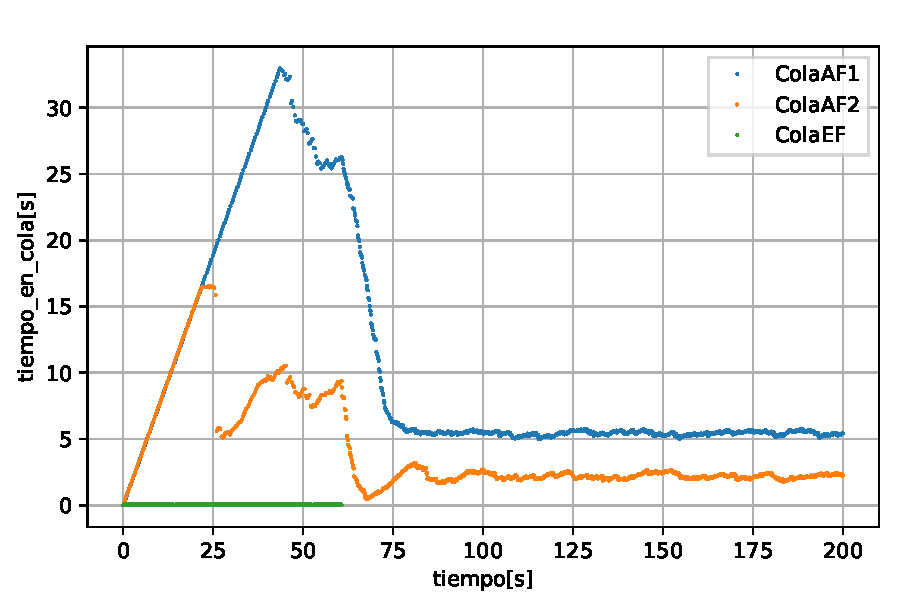
\includegraphics{graficas/RED/tiempo_en_cola_red.pdf}
    \caption{Tiempo encolado cola del router con QoS usando colas RED}
    \label{fig:colasRED_time}
\end{figure}

\subsection{Explica las ventajas e inconvenientes del comportamiento de cada cola AF1x y AF2x. }

En la cola \textbf{AFX1}, la ventaja es que al tener el umbral máximo alto, el nº de paquetes que se pierden es poco y además tiene una probabilidad
de descarte flexible. Como inconveniente es que el tiempo de encolado de paquetes es mayor que \textbf{AFX2}, por lo se tardan más en transmitir.

Con respeto a la cola \textbf{AFX2}, la principal ventaja es el tiempo de encolado, ya que es bajo. 
Los inconvenientes son que al principio, el nº de paquetes decartados son muy seguidos ya que tiene una alta probabilidad de descarte y además el
umbral máximo está por debajo del tamaño de la cola por lo que se están desperdiciando recursos y como conseuencia la cola se llena más rápido.
 

